\documentclass[border=2mm]{standalone}

\usepackage{amsmath}
\usepackage{pgfplots}
\pgfplotsset{compat=1.18}
\usetikzlibrary{arrows.meta, calc, positioning, decorations.pathreplacing, calligraphy}

\usepackage{xcolor}
\definecolor{den-1}{HTML}{111111}   % Đen #111111
\definecolor{den-2}{HTML}{222222}   % Đen #222222
\definecolor{den-3}{HTML}{333333}   % Đen #333333
\definecolor{den-4}{HTML}{444444}   % Đen #444444
\definecolor{den-5}{HTML}{555555}   % Đen #555555
\definecolor{den-6}{HTML}{666666}   % Đen #666666

\tikzset{
  >=Stealth,
  originlabel/.style={
    font=\small\sf,
    anchor=north east, 
    yshift=-0.1ex,     
    xshift=-0.1ex      
  }
}

\begin{document}

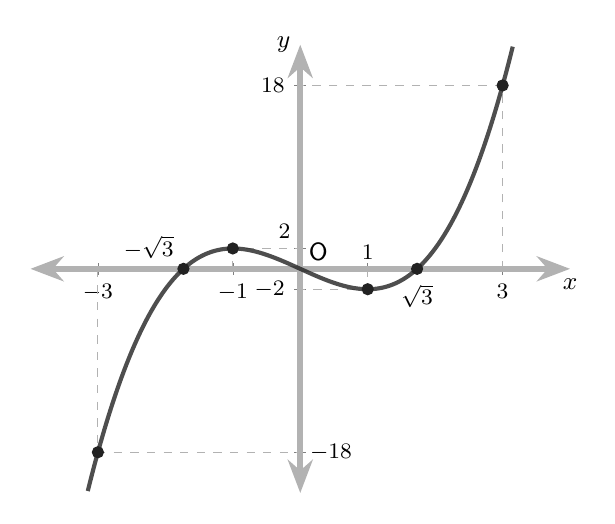
\begin{tikzpicture}

\begin{axis}[
    font=\small\sf,
    axis lines=middle,
    axis line style={<->, line width=2pt, color=den-6!50},
    xlabel=$x$, ylabel=$y$,
    xlabel style={below, font=\small\sf},
    ylabel style={left, font=\small\sf},
    xmin=-4, xmax=4,
    ymin=-22, ymax=22,
    xtick={-3, -1.732, -1, 1, 1.732, 3},
    ytick={-18, -2, 2, 18},
    xticklabels={$-3$, , $-1$, , $\sqrt{3}$, $3$},
    yticklabels={, $-2$, , $18$},
    tick label style={font=\footnotesize\sf},
    % xscale=1,
    % yscale=2,
    clip=false,
]

\node[originlabel] at (axis cs:0,0) [anchor=south west] {O};

\node at (axis cs:1,0) [anchor=south] {\footnotesize $1$};

% \node at (axis cs:0,-2) [anchor=north east] {\footnotesize $-2$};

\node at (axis cs:0,2) [anchor=south east] {\footnotesize $2$};

\node at (axis cs:0,-18) [anchor=west] {\footnotesize $-18$};

\node at (axis cs:-1.732,0) [anchor=south east] {\footnotesize $-\sqrt{3}$};

\draw [dashed, color=den-6!50] (3,0) -- (3,18) -- (0,18);
\draw [dashed, color=den-6!50] (-3,0) -- (-3,-18) -- (0,-18);
\draw [dashed, color=den-6!50] (1,0) -- (1,-2) -- (0,-2);
\draw [dashed, color=den-6!50] (-1,0) -- (-1,2) -- (0,2);

\addplot[domain=-3.15:3.15, samples=200, line width=1.5pt, color=den-2, opacity=.8] {x^3-3*x};

\addplot [only marks, mark=*, color=den-2, mark size=2pt] coordinates {
  (-3, -18)
  (-1.732, 0)
  (-1, 2)
  (1, -2)
  (1.732, 0)
  (3, 18)
};

\end{axis}

\end{tikzpicture}

\end{document}
